%%% VCU thesis/dissertation template file
\makeatletter
\let\my@xfloat\@xfloat
\makeatother

\documentclass[reqno]{vcuthesis}
\makeatletter
\def\@xfloat#1[#2]{
        \my@xfloat#1[#2]%
        \def\baselinestretch{1}%
        \@normalsize \normalsize
}
\makeatother
%%%%%%%%%%%%
% PACKAGES %
\usepackage{bm,amsmath,subfigure,graphicx,url,algorithm,algorithmicx,algpseudocode,booktabs}
\usepackage{tikz-cd,adjustbox,amsfonts,mathtools,tabularx,capt-of,longtable,comment,caption}
\usepackage[flushleft]{threeparttable}
\usepackage[top=1in,bottom=1in,right=1in,left=1in]{geometry}
\usepackage[backend=bibtex]{biblatex}
\usepackage[titletoc]{appendix}
\usepackage{pgfplots}
\pgfplotsset{compat=1.12}
\usepackage[linktocpage=true]{hyperref}
\usetikzlibrary{shapes.geometric,arrows,automata,positioning}
\usepackage{chngcntr}
\usepackage[final]{pdfpages}
\usepackage[explicit]{titlesec}

\newcommand{\iitem}{\item[-]}
\newcommand{\set}[1]{{\left\{#1\right\}}} 
\newcommand{\norm}[1]{{||#1||}} 
\newcommand{\st}{{\,|\,}} 
\newcommand{\reals}{{\mathbb{R}}}
\newcommand{\ints}{{\mathbb Z}}
\newcommand{\spa}[1]{\mathcal{#1}}
\newcommand\tab[1][1cm]{\hspace*{#1}}
\newcommand{\Rho}{\mathrm{P}}

%%%%%%%%%%%
\overfullrule=5pt
% BIBLIOGRAPHY %
\bibliography{references}
\renewcommand{\type}{Dissertation}
\renewcommand{\thetable}{\arabic{table}}
\newcommand{\comments}[1]{}
%%%%%%%%%%%

% EQUATIONS %
\numberwithin{equation}{chapter}
%%%%%%%%%%%

% DOCUMENT  %
\begin{document}
\counterwithin{figure}{chapter}
\counterwithin{algorithm}{chapter}
\counterwithin{table}{chapter}

\pagenumbering{roman}

\makeatletter
\newcommand\pagenumberingnoreset[1]{\gdef\thepage{\csname @#1\endcsname\c@page}}
\makeatother

\tikzstyle{decision} = [diamond, draw, text centered, inner sep=3pt]
\tikzstyle{block} = [rectangle, draw, fill=gray!20,text width=5em, text centered, rounded corners, minimum height=4em]
\tikzstyle{arrow} = [thick,->,>=stealth]

%%%%%%%%%%%
\newcommand{\thesisordissertation}{Dissertation}
\newcommand{\thesistitle}{\uppercase\expandafter{} Novel Support Vector Machines for Diverse Learning Paradigms}
\newcommand{\authorsname}{Gabriella Angela Melki}
\newcommand{\thesismonth}{September}
\newcommand{\graduatingyear}{2018}
\newcommand{\degree}{Doctor of Philosophy}
\newcommand{\pastdegreeone}{Ph.D. Candidate}
\newcommand{\pastdegreetwo}{MSc. Computer Science, Virginia Commonwealth University, 2016} % 897 in .cls
\newcommand{\committeechair}{Alberto Cano}
\newcommand{\committeechairtwo}{Sebastian Ventura}
\newcommand{\major}{Computer Science}
\newcommand{\school}{Virginia Commonwealth University}
\newcommand{\chairposition}{Assistant Professor}
\newcommand{\chairpositiontwo}{Professor}
\newcommand{\majortwo}{Computer Science \& Numerical Analysis}
\newcommand{\schooltwo}{University of C\'{o}rdoba}

\vspace*{10em}
\begin{center}
\thispagestyle{empty}
\copyright Gabriella Angela Melki, September {\graduatingyear}\\
All Rights Reserved.
\end{center}
\vspace*{\fill}
\maketitlepage

\setlength{\headheight}{12pt}

\chapter{Multi-Target SVR using Maximum Correlation Chains}
This contribution presents three multi-target support vector regression (SVR) models. The first involves building independent, single-target SVR models for each output variable. The second builds an ensemble of random chains using the first method as a base model, named SVR with Random Chains (SVRRC), inspired by the classification MT method, Ensemble of Random Chains Corrected (ERCC)~\cite{Spyromitros2014}. The third calculates the targets' correlations and forms a maximum correlation chain, which is used to build a single chained model named SVR with Correlation Chaining (SVRCC). The experimental study compares the performance of the three approaches with six other prominent MT regressors. The experimental results are then analyzed using non-parametric statistical tests. The results show that the maximum correlation SVR approach improves the performance of using ensembles of random chains. 

This chapter is organized as follows: Section~\ref{sec:MTRbackground} describes the notation used throughout this chapter and reviews related works on multi-target regression. Section~\ref{sec:MTRproposal} presents the three multi-target support vector regression approaches. Section~\ref{sec:MTRexperiments} presents the experimental study. Section~\ref{sec:MTRresults} discusses the results and the statistical analysis. Finally, Section~\ref{sec:MTRconclusions} shows the main conclusions of this work.

\section{Multi-Target Regression Background}\label{sec:MTRbackground}
This section first defines the notation that will be used throughout this chapter, and then formally describes the multi-target regression problem along with relevant popular algorithms used within this paradigm.

\subsection{Notation}\label{subsec:mtrnotation}
Let $\mathcal{D}$ be a training dataset of $n$ instances. Let $\bm{X} \in \mathcal{D}$ be a matrix consisting of $d$ input variables and $n$ samples, such that $\bm{X} \in \mathbb{R}^{n \times d}$. Let $\bm{Y} \in \mathcal{D}$ be a matrix consisting of $m$ continuous target variables and $n$ samples,  where $\bm{Y} \in \mathbb{R}^{n \times m}$. 

\subsection{Multi-Target Regression}
In the multi-target learning paradigm, the \textit{problem transformation} approach involves training $m$ independent, single-target models for each target output on datasets $\mathcal{D}_j = \set{\bm X, \bm Y_j},\, \forall j \in \{1, \ldots, m\}$, and is considered as a baseline for measuring model performance~\cite{Spyromitros2014}. Many \textit{problem transformation} methods have been proposed for solve multi-target problems, however, the main issue with this type of approach is that the relationships between the targets is lost once independent models are built for each target. Examples of \textit{problem transformation} approaches include Linear Target Combinations for MT Regression~\cite{Tsoumakas2014}, and Multi-Objective Random Forests (MORF) \cite{Kocev2007}. 

The RC, MTS, MTSC, ERC, and ERCC methods are introduced by Spyromitros et. al. in~\cite{Spyromitros2014}. The idea behind these algorithms was to investigate whether advances in multi-label learning can be successfully used in a multi-target regression setting and shed light on modeling target dependencies. These methods involve two stages of learning, the first being building ST models. The second uses the knowledge gained by the first step to predict the target variables while using possible relationships the targets might have with one another. 

The two stages of training in MTS involve firstly, training $m$ independent single-target models, like in ST. In the second step, a second set of $m$ meta models are learned for each target variable, $\bm{Y}_j,\, 1 \leq j \leq m$. These meta models are learned on a transformed dataset, where the input attributes space is expanded by adding the approximated target variables obtained in the first stage, excluding the $j^{th}$ target being predicted.

The ERC method is somewhat similar to the MTS method. In the training of a Regression Chain (RC) model, a random chain, or sequence, of the set of target variables is selected and for each target in the chain, models are built sequentially by using the output of the previous model as input for the next~\cite{Xioufis2016}. If the default, ordered chain is $C = \{\bm Y_1, \bm Y_2, \ldots, \bm Y_m\}$, the first model $h_1 : \bm X \rightarrow \mathbb{R}$ is trained for $\bm Y_1$, as in ST. For the subsequent models $h_{j,j>1}$, the dataset is transformed by sequentially appending the true values of each of the previous targets in the chain to the input vectors. For a new input vector, the target values are unknown. So once the models are trained, the unseen input vector will be appended with the approximated target values, making the models dependent on the approximated values obtained in each step. One of the issues associated with this method is that, if a single random chain is used, the possible relationships between the targets at the head of the chain and the end of the chain are not exploited due to the algorithm's sequential nature. Also, prediction error in the earlier stages of the models will be propagated as the rest of the models are trained, which is why the Ensemble of Regressor Chains was proposed in ~\cite{Spyromitros2014}. Instead of a single chain, $k$ chains are created at random, and the final prediction values are obtained by taking the mean values of the $k$ predicted values for each target. 

In the methods described above, the estimated target variables (meta-variables) are used as input in the second stage of training. In both methods, the models are trained using these meta-variables that become noisy at prediction time, and thus the relationship between the meta-variables and target variable is muddied. Dividing the training set into sets, one for each stage, would not help this situation because both methods would be trained on training sets of decreasing size. Due to these issues, \textit{Spyromitros et. al.} proposed modifications, in \cite{Spyromitros2014}, to both methods that resembles $k$-fold cross-validation (CV) to be able to obtain unbiased estimates of the meta-variables. These methods are called Regression Chains Corrected (RCC) and Multi-Target Stacking Corrected (MTSC). 

The ERCC and MTSC procedures involve repeating the RCC and MTS procedures $k$ times, respectively, with $k$ randomly ordered chains for ERCC, and $k$ different modified training sets for MTSC. The algorithms were tested and compared using Bagging of $100$ regression trees as their base regression algorithm with ERC and ERCC ensemble size of $10$, and $10$-fold cross-validation. The corrected methods exhibited better performance than their original variants, as well as ST models. The ERCC algorithm had the best overall performance, as well as being statistically significantly more accurate of all the methods tested. These methods can be found and used through the open-source Java library, Mulan~\cite{mulan}; to replicate the results found in~\cite{Spyromitros2014}.

\section{Three Novel SVMs for Multi-Target Regression}\label{sec:MTRproposal}
Three novel models have been implemented for the purposes of multi-target regression. The base model is the SVR model, where $m$ single-target soft margin non-linear support vector regressors (NL-SVR) are built for each target variable $\bm Y_j$. 
\begin{figure}[b!]
\begin{minipage}{0.9\textwidth}
\small \centering
\[\begin{tikzcd}[column sep = small, row sep = small]
& & \mathcal{D}_1 :  [\bm X][\bm Y_1]  \arrow[rr]  & & h_1 :  \mathcal{D}_1 \rightarrow \bm{\hat{Y_1}}\\
& & \mathcal{D}_2 :  [\bm X][\bm Y_2]  \arrow[rr] & & h_2 :  \mathcal{D}_2 \rightarrow \bm{\hat{Y_2}} \\        
\mathcal{D} :  [\bm X][\bm Y]  \arrow[uurr, bend left=45] \arrow[urr, bend left] \arrow[drr, bend right]  		& & \vdots \\
& & \mathcal{D}_m :  [\bm X][\bm Y_m] \arrow[rr] & & h_m :  \mathcal{D}_m \rightarrow \bm{\hat{Y}_m}
\end{tikzcd}\]
\end{minipage}
\caption{SVR Flow Diagram. Firstly, the SVR method divides the MT dataset into $m$ ST datasets, $\mathcal{D}_1, \mathcal{D}_2, \ldots, \mathcal{D}_m$. It then independently trains models, $h_1, h_2, \ldots, h_m$, for each ST dataset.}\label{diag:SVR}
\begin{algorithm}[H]
\caption{MT Support Vector Regression (SVR)} \label{alg:SVR} 
\small \centering
\begin{algorithmic}[1]
\renewcommand{\algorithmicrequire}{\textbf{Input:}}
\renewcommand{\algorithmicensure}{\textbf{Output:}}
\Require Training dataset $\mathcal{D}$
\Ensure  ST models $h_j, j = 1,\ldots,m$
\For {$j = 1$ to $m$}
\State $\mathcal{D}_j = \{\bm X, \bm Y_j\}$ \Comment{Get ST data}
\State $h_j : \bm X \rightarrow \mathbb{R}$ \Comment{Build ST model for the $j^{th}$ target}
\EndFor \\
\Return $h_j, j=1,\ldots,m$ 
\end{algorithmic} 
\end{algorithm}
\end{figure}

For NL-SVR, the regularized soft margin loss function given in equation~\eqref{eq:softsvropt} is minimized. This contribution involves solving the dual of this formulation given by \eqref{eq:dualSVR}. Using the dual formulation, the multi-target problem is solved by transforming it into $m$ single-target problems, as shown in Algorithm~\ref{alg:SVR} and Figure~\ref{diag:SVR}. This algorithm will output $m$ single-target models, $h_j,\,\forall j = 1,\ldots,m$, for a given dataset $\mathcal{D}$. It first splits the dataset into $m$ separate ones, $\mathcal{D}_j$, each with a single-target variable $\bm Y_j$, and then builds a distinct SVR model for each of the datasets. 

Building $m$ ST models is a good base-line, but as mentioned previously, it does not capture possible correlations between the target attributes during training. If these correlations are not exploited, this could retract from the model's potential performance. Therefore, creating an ensemble model using a series of random chains was proposed, using the base-line SVR method, named SVR Random Chains (SVRRC). 
\begin{algorithm}[t!]
\centering \small
\caption{Build Chained Model}
\label{alg:buildchainedmodel} 
\begin{algorithmic}[1]
\renewcommand{\algorithmicrequire}{\textbf{Input:}}
\renewcommand{\algorithmicensure}{\textbf{Output:}}
\Require Training dataset $\mathcal{D}$, random chain $\bm C$
\Ensure  A chained model $h_j, j = \{1,\ldots,m\}, c \leq 10$
\State $\mathcal{D}_1 = \set{\bm X, \bm Y_{\bm C_1}}$ \Comment{Initialize first dataset}
\For {$j=1$ to $m$} \Comment{For each target in chain $\bm C$}
\State $h_j : \mathcal{D}_j \rightarrow \mathbb{R}$ \Comment{Train model on appended dataset}
\If {$j < m$}
\State $\mathcal{D}_{j+1} = \set{\mathcal{D}_j, \bm Y_{\bm C_j}}$ \Comment{Append new target in chain to dataset}
\EndIf
\EndFor \\
\Return $h_j, j=1,\ldots,m$ 
\end{algorithmic} 
\end{algorithm}

For SVRRC, ensembles of at most $10$ $m$-sized random chains, $\mathcal{C}$, are built from different and distinct permutations of the target variable indices. When chaining target values, there are two main options: using the predicted value as input for the following target, or using the true value of the target variable as input of the subsequent targets. The main problem with the former approach is that errors are propagated throughout the chained model, therefore SVRCC employs chaining of the true values. 

For each random chain, a new model is trained by predicting the first target variable in the chain. Next, the first target's true value, $\bm Y_j$, is appended to the training set. This chaining process is repeated for all the target indices in the chains, $\{\bm C_1, \ldots, \bm C_c\} \in \mathcal{C}, \, c \leq 10 \,$. This process will be repeated for each random chain generated, returning an ensemble of chained SVRs. Algorithm~\ref{alg:buildchainedmodel} describes the process of building a chained model given chain $\bm C \in \mathcal{C}$, and Algorithm~\ref{alg:SVRRC} shows the steps taken by SVRRC. 

Given this ensemble of chained models, the predicted values for a given unseen instance are calculated by taking the mean of the multiple models generated using different random chains. Since the unseen input has no known target value, the predicted value at each step of the chain $\hat{\bm Y}_j$ is appended to the input at each step of the chain. 
\begin{figure}[t]
\centering \small
\begin{minipage}{\textwidth}
\centering \small
\begin{tikzcd}[column sep = small, row sep = small]
& \mathcal{D} :  [\bm X][\bm Y_1 \bm Y_2 \bm Y_3] \arrow[dl] \arrow[d] \arrow[drr] & & \\
\left[1,2,3\right] \arrow[d] & \left[1,3,2\right] \arrow[d] & \hdots & \left[3,2,1\right] \arrow[d] \\
h_1 :  [\bm X] \rightarrow \bm{\hat{Y_1}} \arrow[d] & h_1 :  [\bm X] \rightarrow \bm{\hat{Y_1}} \arrow[d] & \hdots & h_1 :  [\bm X] \rightarrow \bm{\hat{Y_1}} \arrow[d] \\
h_2 :  [\bm X \bm{Y_1} ] \rightarrow \bm{\hat{Y_2}} \arrow[d] & h_2 :  [\bm X \bm{Y_1} ] \rightarrow \bm{\hat{Y_3}} \arrow[d] & \hdots & h_2 :  [\bm X \bm{Y_3} ] \rightarrow \bm{\hat{Y_2}} \arrow[d] \\
h_3 :  [\bm X \bm{Y_1Y_2} ] \rightarrow \bm{\hat{Y_3}} & h_3 :  [\bm X \bm{Y_1Y_3} ] \rightarrow \bm{\hat{Y_2}} & \hdots & h_3 :  [\bm X \bm{Y_3Y_2} ] \rightarrow \bm{\hat{Y_1}}
\end{tikzcd}
\end{minipage}
\caption{SVRRC Flow Diagram on a dataset with 3 targets. SVRRC first builds the $6$ random chains of the target's indices ($3$ examples are shown). It then constructs a chained model by proceeding recursively over the chain, building a model, and appending the current target to the input space to predict the next target in the chain. } \label{fig:svrrc}
\begin{algorithm}[H]
\caption{MT SVR with Random-Chains (SVRRC)}
\small \centering
\label{alg:SVRRC} 
\begin{algorithmic}[1]
\renewcommand{\algorithmicrequire}{\textbf{Input:}}
\renewcommand{\algorithmicensure}{\textbf{Output:}}
\Require Training dataset $\mathcal{D}$, $c$ random chains $\mathcal{C}$
\Ensure  An ensemble of chained models $h_\mathcal{C}$
\For {\textbf{each }$\bm C \in \mathcal{C}$} \Comment{For each random chain}
\State $h_{\bm C} = $ \text{build chained model}$(\mathcal{D},\bm C)$ \Comment{build a chained model for chain $\bm C$}
\EndFor \\
\Return $h_\mathcal{C}$ 
\end{algorithmic} 
\end{algorithm}
\end{figure}

Due to the computational complexity of building $m!$ distinct chains and training $\left(m!\right) \times m$ models, the number of ensembles and chains are limited to a maximum of $10$. However, if the number of target variables is less than $3$, i.e. $m! \leq 10$, all $m!$ random chains are constructed. 

A disadvantage of building an ensemble of 10 random chains stems from the fact that: when the number of output variables increases, the number of possible chains increases factorially. Therefore, there is no guarantee that the 10 random chains generated will truly reflect the relationships among the target variables. Additionally, building an ensemble of regressors is computationally expensive. Finding a heuristic that allows the identification of a single, most appropriate chain, which fully reflects the output variable interrelations would improve the scalability of training the ensemble. 

The third proposal was designed to remedy this issue. It builds a single chain based on the maximization of the correlations among the target variables. By calculating the correlation of the target variables and imposing it on the order of the chain, this ensures that each appended target provides some additional knowledge on the training of the next. With SVRRC, there is no reasoning behind the generation of these chains, and since the number of random chains generated is limited to $10$, there is no way of ensuring that the $10$ chains fully represent the targets' dependencies. Calculating and using the correlations of the targets would break this uncertainty. Algorithm~\ref{alg:SVRCC} presents the SVR Correlation Chain (SVRCC) method. The computational complexity and hardware constraints (memory size) are negligible during the construction of the targets' correlation matrix, since the correlation matrix would be an $(m \times m)$ matrix, and the likelihood that the number of targets is large enough to cause a memory issue is minimal. 
\begin{figure}[t]
\begin{minipage}{\textwidth}
\centering \small
\begin{tikzcd}
\mathcal{D} :  [\bm X][\bm Y_1 \bm Y_2 \bm Y_3] \arrow{rr}{\textit{generate maximum correlation chain}}[swap]{\frac{\mathbf{E}\left[(Y_i - \mu_i)(Y_j - \mu_j)\right]}{\sqrt{\mathbf{E}\left[(Y_i - \mu_i)(Y_i - \mu_i)\right]\mathbf{E}\left[(Y_j - \mu_j)(Y_j - \mu_j)\right]}}} 
&  \arrow[d, phantom, ""{coordinate, name=Z}]
& \left[1,2,3\right]  \arrow[dll, rounded corners, to path={ -- ([xshift=1ex]\tikztostart.east)
|- ([yshift=-2.5ex]Z) [near end]\tikztonodes
-| ([xshift=-1ex]\tikztotarget.west)
-- (\tikztotarget)}] \\
h_1 :  [\bm X] \rightarrow \bm{\hat{Y_1}} \arrow[r]
& h_2 :  [\bm X \bm{Y_1} ] \rightarrow \bm{\hat{Y_2}} \arrow[r]
& h_3 :  [\bm X \bm{Y_1Y_2} ] \rightarrow \bm{\hat{Y_3}} 
\end{tikzcd}
\end{minipage}
\caption{SVRCC Flow Diagram on a sample dataset with 3 targets. SVRCC first finds the direction of maximum correlation among the targets and uses that order as the only chain. It then constructs the chained model as done in SVRRC. } \label{fig:svrcc}
\begin{algorithm}[H]
\caption{MT SVR with Max-Correlation Chain (SVRCC)} \label{alg:SVRCC} 
\centering \small
\begin{algorithmic}[1]
\renewcommand{\algorithmicrequire}{\textbf{Input:}}
\renewcommand{\algorithmicensure}{\textbf{Output:}}
\State $\bm \Rho = corrcoef(\bm Y)$ \Comment{Find correlation coefficient matrix for target variables}
\State $\bm C = \sum_{i=1}^n \bm \Rho_{ij}, \forall j=1,\ldots,m$ \Comment{Sum row elements of the correlation coefficient matrix}
\State $\bm C = \text{sort}\left(\bm C,\textbf{decreasing}\right)$ \Comment{Sort sums in decreasing order}
\State $h_{\bm C} = $ \text{build chained model}$(\mathcal{D},\bm C)$ \Comment{build a chained model for max correlation chain $\bm C$} \\
\Return $h_{\bm C}$
\end{algorithmic} 
\end{algorithm}
\end{figure}

To calculate the correlation coefficients of the targets, the targets' co-variance matrix, $\bm \Sigma$, is first calculated as shown in Equation~\ref{eq:corr}:
\begin{equation}
\label{eq:corr}
\centering
\bm \Sigma_{ij} = cov(\bm Y_i,\bm Y_j) = \mathbf{E}\left[(\bm Y_i - \mu_i)(\bm Y_j - \mu_j)\right],
\end{equation}
where $\mu_i = \mathbf{E}(\bm Y_i)$, and $\mathbf{E}(\bm Y_i)$ is the expected value of $\bm Y_i$, $\forall i,j \in \{1,\ldots,m\}$. This matrix will show how the targets change together. 

The correlation coefficients matrix, $\bm \Rho$, is then calculated as shown in Equation~\ref{eq:corrcoef}:
\begin{equation}
\label{eq:corrcoef}
\centering
\bm \Rho = corrcoef(\bm Y) = \frac{\bm \Sigma_{ij}}{\sqrt{\bm \Sigma_{ii}\bm \Sigma_{jj}}},\, \forall i,j \in \{1,\ldots,m\}.
\end{equation}
It will describe the linear relationship among the target variables. The coefficients are then sorted in decreasing order, creating the maximum correlation chain. 

\section{Experimental Environment}\label{sec:MTRexperiments}
Although many interesting applications of multi-target regression exist, there are not many publicly available datasets to use. The datasets used in the experimental study were collected from the Mulan website~\cite{mulan}, as well as the UCI Machine Learning Repository~\cite{Lichman:2013}. Information on the $24$ datasets used is summarized in Table~\ref{tab:mtrdatasets}, where the number of samples, attributes (dimensionality), and targets are shown. 
\begin{table}[t!]
\centering \small
\caption{Multi-Target (MT) Regression datasets} \label{tab:mtrdatasets}
\begin{tabular}{lccc}
\noalign{\smallskip}\hline\noalign{\smallskip}
Dataset & Samples $(n)$ & Attributes $(d)$ & Targets $(m)$\\
\noalign{\smallskip}\hline\noalign{\smallskip}
EDM & 145 & 16 & 2\\
Enb & 768 & 8 & 2 \\
Jura & 359 & 11 & 7 \\
Osales & 639 & 413 & 12 \\
Scpf & 1137 & 23 & 3 \\
Slump & 103 & 7 & 3 \\
Solar Flare 1 & 323 & 10 & 3\\
Solar Flare 2 & 1,066 & 10 & 3\\
Water Quality & 1,060 & 16 & 14\\
OES97 & 323 & 263 & 16\\
OES10 & 403 & 298 & 16\\
ATP1d & 201 & 411 & 6\\
ATP7d & 188 & 411 & 6\\
Andro & 49 & 30 & 6 \\
Wisconsin Cancer & 198 & 34 & 2\\
Stock & 950 & 10 & 3\\
California Housing & 20,640 & 7 & 2\\
Puma8NH & 8,192 & 8 & 3\\
Puma32H & 8,192 & 32 & 6\\
Friedman & 500 & 25 & 6\\
Polymer & 41 & 10 & 4\\
M5SPEC & 80 & 700 & 3\\
MP5SPEC & 80 & 700 & 3\\
MP6SPEC & 80 & 700 & 3\\
\noalign{\smallskip}\hline\noalign{\smallskip}
\end{tabular}
\end{table}

Experiments were performed over the RC, ST, MTS, MTSC, ERC, ERCC, and MORF algorithms, which have also been used in the experimental study conducted in~\cite{Spyromitros2014}. These algorithms were chosen because they have shown considerable performance in training multi-target models. The have also made their framework readily available for reproducing their results. All three SVR algorithms are implemented within the general framework of Mulan's MTRegressor\footnote{http://mulan.sourceforge.net}~\cite{mulan}, which was built on top of Weka\footnote{http://www.cs.waikato.ac.nz/ml/weka}~\cite{Hall2009}. LIBSVM's Epsilon-SVR~\cite{CC01a} implementation was used as the base SVR model. The parameters experimented with for the SVR regression task are the penalty parameter $C$, the Gaussian kernel parameter $\gamma$, and the error or tube parameter $\epsilon$ given by Equations~\eqref{eq:paramCmtr} to~\eqref{eq:paramE}, referred to as~\eqref{eq:hyperparammtr}.
\begin{subequations}
\label{eq:hyperparammtr}
\begin{align}
C \in  & \{1, 10, 100\} \label{eq:paramCmtr}\\
\gamma \in  & \{1^{-9}, 1^{-7}, 1^{-5}, 1^{-3}, 1^{-1}, 1, 5, 10\} \label{eq:mtrparamG}\\
\epsilon \in  & \{0.01, 0.1, 0.2\} \label{eq:paramE}
\end{align}
\end{subequations}

To ensure a controlled environment when conducting the performance comparisons, the experimental environment for running the competing algorithms was the same as what was done in~\cite{Spyromitros2014}. This includes the following. The ST base-line model used was Bagging~\cite{Breiman1996} of 100 regression trees~\cite{Wu2015430}. The MTSC and ERCC methods are run using $10$-fold cross-validation, and the ensemble size for the ERC and ERCC methods was set to $10$. The ensemble size of 100 trees was used for MORF, and the rest of its parameters were set as recommended by~\cite{Kocev2013}.

The performance metrics used to analyze our contributions' performances are shown in Equations~\ref{eqn:aCC} to~\ref{eqn:arrmse}. For unseen or test datasets of size $\mathcal N_{test}$, the performances are evaluated by taking the run time (seconds) each algorithm takes to build a classifier, as well as the following metrics, where the upwards arrow $\uparrow$ indicates maximizing the metric and the downwards arrow $\downarrow$ indicates minimizing the metric.

\begin{itemize}
\item The average correlation coefficient (aCC $\uparrow$):
\begin{eqnarray}
\frac{1}{m} \sum_{j = 1}^m \frac{\sum_{l = 1}^{\mathcal N_{test}} (y_j^{(l)} - \bar{y}_j)(\hat{y}_j^{(l)} - \bar{\hat{y}}_j)}{\sqrt{\sum_{l = 1}^{\mathcal N_{test}} (y_j^{(l)} - \bar{y}_j)^2 \sum_{l = 1}^{\mathcal N_{test}} (\hat{y}_j^{(l)} - \bar{\hat{y}}_j)^2}}
\label{eqn:aCC}
\end{eqnarray}

\item The mean squared error (MSE $\downarrow$):
\begin{eqnarray}
\frac{1}{m} \sum_{j = 1}^m \frac{1}{\mathcal N_{test}} \sum_{l = 1}^{\mathcal N_{test}} (y_j^{(l)} - \hat{y}^{(l)}_j)^2
\label{eqn:MSE}
\end{eqnarray}

\item The average root mean squared error (aRMSE $\downarrow$):
\begin{eqnarray}
\frac{1}{m} \sum_{j = 1}^m \sqrt{\frac{\sum_{l = 1}^{\mathcal N_{test}} (y_j^{(l)} - \hat{y}^{(l)}_j)^2}{\mathcal N_{test}}}
\label{eqn:armse}
\end{eqnarray}

\item The average relative root mean squared error (aRRMSE $\downarrow$):
\begin{eqnarray}
\frac{1}{m} \sum_{j = 1}^m \sqrt{\frac{\sum_{l = 1}^{\mathcal N_{test}} (y_j^{(l)} - \hat{y}_j^{(l)})^2}{\sum_{l = 1}^{\mathcal N_{test}} (y_j^{(l)} - \bar{y}_j)^2}}
\label{eqn:arrmse}
\end{eqnarray}
\end{itemize}

The predicted output is represented by $\hat{\textbf{y}}$, the average of the predicted output is $\bar{\hat{\textbf{y}}}$, and the average of the true output target variable is $\bar{\textbf{y}}$. The test dataset is the hold-out set during cross validation. This ensures our model is evaluated on data that it has not been trained on, and thus unbiased towards the training datasets. It also contributes to the generalizability and robustness of the model.

\section{Results \& Statistical Analysis}\label{sec:MTRresults}
Tables~{\ref{tab:mtraccResults}},~{\ref{tab:mseResults}},~{\ref{tab:armseresults}},~{\ref{tab:arrmseresults}}, and~{\ref{tab:timeresults}} show the results of our algorithm implementations compared with those of \textit{RC, MORF, ST, MTS, MTSC, ERC,} and \textit{ERCC}. Each subsection discusses a single metric along with the statistical analysis of the results. The best metric value obtained on each dataset is typeset in bold. Non-parametric statistical tests are then used to validate the experiments results obtained. To determine whether significant differences exist among the performance and results of the algorithms, the Iman-Davenport non-parametric test is run to rank the algorithms over the datasets used, according to the Friedman test. The average ranks are presented in the last row of the results tables. The Bonferroni-Dunn post-hoc test~{\cite{Dunn1961}} is then used to find these differences that occur between the algorithms. Below each result table, a diagram highlighting the critical distance (in gray) between each algorithm is shown. The Wilcoxon, Nemenyi, and Holm~{\cite{Wilcoxon1945}} tests were run for each of the result metrics to compute multiple pairwise comparisons among the algorithms used in the experimental study. Tables~{\ref{tab:statacc}},~{\ref{tab:statmse}},~{\ref{tab:statarmse}},~{\ref{tab:statarrmse}}, and~{\ref{tab:stattime}} show the sum of ranks $R^+$ and $R^-$ of the Wilcoxon rank-sum test, and the $p$-values for the $3$ tests, which show the statistical confidence rather than using a fixed $\alpha$ value.

\subsection{Average Correlation Coefficient}\label{subsec:acc}
\begin{table}[t!]
\centering \small
\caption{Average Correlation Coefficient (aCC) for MT regressors}\label{tab:mtraccResults}
\resizebox{0.95\textwidth}{!}{\begin{tabular}{l@{\extracolsep{\fill}}ccccccccccc}
\noalign{\smallskip}\hline\noalign{\smallskip}
Datasets &MORF &ST &MTS &MTSC &RC &ERC &ERCC &SVR &SVRRC &SVRCC \\
\noalign{\smallskip}\hline\noalign{\smallskip}
Slump &0.6965 &0.7062 &0.7163 &0.6977 &0.6956 &0.6977 &0.7023 &0.7245 &0.7339 &\textbf{0.7457} &  \\
Polymer &0.7305 &0.7336 &0.7371 &0.7228 &0.7015 &0.7029 &0.7222 &0.7634 &0.7857 &\textbf{0.7905} &  \\
Andro &\textbf{0.7349} &0.6454 &0.6793 &0.6581 &0.6915 &0.6806 &0.6653 &0.6880 &0.6951 &0.7056 &  \\
EDM &\textbf{0.6722} &0.6352 &0.6412 &0.6354 &0.6355 &0.6379 &0.6354 &0.6484 &0.6565 &0.6567 &  \\
Solar Flare 1 &0.1083 &0.1258 &0.1034 &0.1193 &\textbf{0.1492} &0.1387 &0.1292 &0.1066 &0.0857 &0.1152 &  \\
Jura &0.7854 &0.7907 &0.7880 &0.7882 &0.7877 &0.7884 &0.7897 &0.7789 &0.7921 &\textbf{0.7983} &  \\
Enb &0.9828 &0.9832 &0.9822 &0.9829 &0.9813 &0.9823 &0.9837 &0.9858 &0.9867 &\textbf{0.9868} &  \\
Solar Flare 2 &0.2357 &0.2295 &0.2375 &0.2343 &0.2302 &0.2351 &\textbf{0.2432} &0.1470 &0.1648 &0.1656 &  \\
Wisconsin Cancer &0.3362 &0.3587 &\textbf{0.3652} &0.3588 &0.3628 &0.3609 &0.3590 &0.3187 &0.3208 &0.3373 &  \\
California Housing &0.7705 &0.7720 &0.7149 &0.7451 &0.7007 &0.7844 &\textbf{0.8065} &0.7847 &0.7949 &0.8007 &  \\
Stock &0.9785 &0.9747 &0.9755 &0.9752 &0.9753 &0.9757 &0.9763 &0.9825 &\textbf{0.9829} &0.9822 &  \\
SCPF &0.5827 &0.5508 &0.5503 &0.5477 &0.5569 &0.5656 &0.5515 &0.5891 &\textbf{0.5975} &0.5946 &  \\
Puma8NH &0.5424 &0.4828 &0.4942 &0.4205 &0.4677 &0.4656 &0.4650 &\textbf{0.6041} &0.5975 &0.6038 &  \\
Friedman &0.1507 &0.1609 &0.1548 &0.1667 &0.1558 &0.1608 &0.1632 &0.1710 &0.1748 &\textbf{0.1752} &  \\
Puma32H &0.3085 &0.2934 &0.2890 &0.2504 &0.2754 &0.2870 &0.2797 &0.3358 &0.3351 &\textbf{0.3385} &  \\
Water Quality &\textbf{0.4303} &0.4063 &0.4019 &0.4051 &0.3992 &0.4052 &0.4147 &0.3545 &0.3828 &0.3857 &  \\
M5SPEC &0.8161 &0.8346 &0.8134 &0.8228 &0.8333 &0.8340 &0.8308 &0.9451 &0.9452 &\textbf{0.9472} &  \\
MP5SPEC &0.8315 &0.8536 &0.8244 &0.8535 &0.8524 &0.8526 &0.8542 &0.9560 &0.9602 &\textbf{0.9633} &  \\
MP6SPEC &0.8317 &0.8531 &0.8231 &0.8531 &0.8507 &0.8515 &0.8541 &0.9444 &0.9500 &\textbf{0.9528} &  \\
ATP7d &0.8260 &0.8408 &0.8422 &\textbf{0.8474} &0.8273 &0.8351 &0.8464 &0.8305 &0.8407 &0.8400 &  \\
OES97 &0.7829 &0.7995 &0.7990 &0.8001 &0.7986 &0.7990 &0.7999 &0.8116 &0.8134 &\textbf{0.8137} &  \\
Osales &0.7186 &0.6912 &0.7104 &0.7076 &0.6357 &0.7136 &\textbf{0.7193} &0.6511 &0.6433 &0.6677 &  \\
ATP1d &0.8961 &0.9066 &0.9051 &0.9075 &0.9048 &0.9081 &0.9071 &0.9092 &\textbf{0.9130} &0.9100 &  \\
OES10 &0.8708 &0.8808 &0.8805 &0.8806 &0.8804 &0.8804 &0.8809 &0.8911 &0.8924 &\textbf{0.8963} &  \\
\noalign{\smallskip}\hline\noalign{\smallskip}
Average &0.6508 &0.6462 &0.6429 &0.6409 &0.6396 &0.6476 &0.6492 &0.6634 &0.6685 &\textbf{0.6739} &  \\
Ranks &6.4167 &5.8958 &6.6042 &6.4792 &7.5208 &5.8958 &4.8542 &4.7917 &3.7083 &\textbf{2.8333} &  \\
\noalign{\smallskip}\hline
\end{tabular}}
\centering \small
\resizebox{0.95\textwidth}{!}{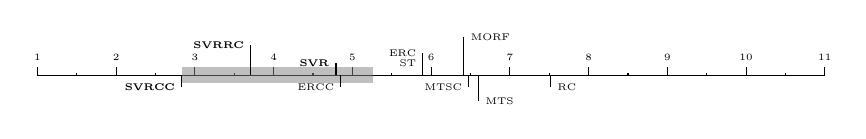
\begin{tikzpicture}
 %axis
 \draw (1,0) -- (11,0);
 \foreach \x in {1,2,3,4,5,6,7,8,9,10,11} {
  \draw (\x, 0) -- ++(0,.1) node [above,scale=0.7] {\tiny \x};
  \ifthenelse{\x < 11}{\draw (\x+.5, 0) -- ++(0,.03);}{}
 }
 % coordinates
 \coordinate (c0) at (2.8333,0);
 \coordinate (c1) at (3.7083,0);
 \coordinate (c2) at (4.7917,0);
 \coordinate (c3) at (4.8542,0);
 \coordinate (c4) at (5.8958,0);
 \coordinate (c5) at (7.5208,0);
 \coordinate (c6) at (6.4792,0);
 \coordinate (c7) at (6.6042,0);
 \coordinate (c8) at (5.8958,0);
 \coordinate (c9) at (6.4167,0);

 % labels
 \node (l0) at (c0) [below left=.025cm and 0cm, align=right, scale=0.7] {\tiny \textbf{SVRCC}};
 \node (l1) at (c1) [above left=.25cm and 0cm, align=right, scale=0.7] {\tiny \textbf{SVRRC}};
 \node (l2) at (c2) [above left=.025cm and 0cm, align=right, scale=0.7] {\tiny \textbf{SVR}};
 \node (l3) at (c3) [below left=.025cm and 0cm, align=left, scale=0.7] {\tiny ERCC};
 \node (l4) at (c4) [above left=.15cm and 0cm, align=right, scale=0.7] {\tiny ERC};
 \node (l5) at (c5) [below right=.025cm and 0cm, align=left, scale=0.7] {\tiny RC};
 \node (l6) at (c6) [below left=.025cm and 0cm, align=right, scale=0.7] {\tiny MTSC};
 \node (l7) at (c7) [below right=.2cm and 0cm, align=left, scale=0.7] {\tiny MTS};
 \node (l8) at (c8) [above left=.025cm and 0cm, align=right, scale=0.7] {\tiny ST};
 \node (l9) at (c9) [above right=.35cm and 0cm, align=right, scale=0.7] {\tiny MORF};

 % CD = 1.4845
 \fill[fill=gray,fill opacity=0.5] (2.8333,-0.1) rectangle (5.2569,0.1);
 
 % connectors
 \foreach \x in {0,...,9} {
  \draw (l\x) -| (c\x);
 };
\end{tikzpicture}}\vspace{-1em}
\captionof{figure}{Bonferroni-Dunn test for aCC}\label{fig:BonfDunnACC}\vspace{-1.5em}
\captionof{table}{Wilcoxon, Nemenyi, and Holm tests for aCC}\label{tab:statacc}
\scriptsize
\resizebox{0.95\textwidth}{!}{\begin{tabular}{lccccc}
\noalign{\smallskip}\hline\noalign{\smallskip}
SVRCC vs. & Wilcoxon $R^{+}$ & Wilcoxon $R^{-}$ & Wilcoxon $p$-value & Nemenyi $p$-value & Holm $p$-value \\ 
\noalign{\smallskip}\hline\noalign{\smallskip}
MORF & 224.0 & 76.0 & $3.4E^{-2}$ & $4.1E^{-5}$& $8.3E^{-3}$ \\
ST & 239.0 & 61.0 & $9.6E^{-3}$ & $4.6E^{-4}$ & $1.3E^{-2}$ \\ 
MTS & 242.0 & 58.0 & $7.2E^{-3}$ & $1.6E^{-5}$ & $6.3E^{-3}$ \\ 
MTSC & 238.0 & 62.0 & $1.1E^{-2}$ & $3.0E^{-5}$ & $7.1E^{-3}$ \\ 
RC & 250.0 & 50.0 & $3.1E^{-3}$ & 0.0000 & $5.6E^{-3}$ \\
ERC & 229.0 & 71.0 & $2.3E^{-2}$ & $4.6E^{-4}$ & $1.0E^{-2}$ \\ 
ERCC & 221.0 & 79.0 & $4.3E^{-2}$ & $2.1E^{-2}$ & $1.7E^{-2}$ \\ 
SVR & 297.0 & 3.00 & $6.0E^{-7}$ & $2.5E^{-2}$ & $2.5E^{-2}$ \\ 
SVRRC & 266.5 & 33.5 & $4.0E^{-4}$ & $3.2E^{-1}$ & $5.0E^{-2}$ \\ 
\noalign{\smallskip}\hline\noalign{\smallskip}
\end{tabular}}
\end{table}
Table~{\ref{tab:mtraccResults}} shows that our proposed methods perform the best on $15$ out of the $24$ datasets. Specifically, the maximum correlation chain method, SVRCC, performs the best on $11$, which is better than the total number of datasets the competing methods performed better at ($9$). The Iman-Davenport statistic, distributed according to the F-distribution with 9 and 207 degrees of freedom is $6.72$, with a $p$-value of $1.9E^{-8}$ which is significantly less than $0.01$, implying a statistical confidence larger than $99\%$. Therefore, we can conclude that there exist statistically significant differences between the aCC results of the algorithms.

Figure~{\ref{fig:BonfDunnACC}} shows the mean rank values of each algorithm along with the critical difference value, $2.4236$, for $\alpha = 0.05$. The algorithms that are to the right of the critical difference rectangle are the ones with significantly different results. Therefore, the $6$ out of $10$ algorithms beyond the critical difference perform significantly worse than our control algorithm, SVRCC. Table~{\ref{tab:statacc}} provides complementary analysis of the results. According to the Wilcoxon test, SVRCC is shown to have significantly better performance over all algorithms with $p$-value $< 0.05$. The Nemenyi and Holm tests show that SVRCC performs significantly better than $6$ out of the $9$ algorithms with $p$-value $\leq 5.6E^{-3}$ and $\leq 1.7E^{-2}$, respectively. The exact confidence for algorithm SVRCC against all others is $0.95$.

\begin{table}[b!]
\centering \small
\caption{Mean Square Error (MSE) for MT regressors}\label{tab:mseResults}
\resizebox{0.95\textwidth}{!}{\begin{tabular}{l@{\extracolsep{\fill}}ccccccccccc}
\noalign{\smallskip}\hline\noalign{\smallskip}
Datasets &MORF &ST &MTS &MTSC &RC &ERC &ERCC &SVR &SVRRC &SVRCC \\
\noalign{\smallskip}\hline\noalign{\smallskip}
Slump &1.4388 &1.4161 &1.3667 &1.4414 &1.4602 &1.4727 &1.4183 &1.2991 &1.1726 &\textbf{1.1614} &  \\
Polymer &1.6718 &1.8120 &1.5446 &1.6726 &1.8259 &1.9999 &1.6873 &1.1874 &1.1068 &\textbf{1.0796} &  \\
Andro &1.4930 &2.1467 &1.4714 &1.7525 &2.2603 &2.0812 &1.8707 &1.5406 &1.2847 &\textbf{1.2187} &  \\
EDM &\textbf{0.8342} &0.9373 &0.9352 &0.9418 &0.9389 &0.9326 &0.9393 &0.9092 &0.8650 &0.8817 &  \\
Solar Flare 1 &3.3458 &3.1196 &3.1193 &3.0524 &3.0357 &3.0381 &3.0594 &\textbf{2.9912} &3.0176 &3.0129 &  \\
Jura &1.0973 &1.0595 &1.0732 &1.0695 &1.0744 &1.0694 &1.0632 &1.1167 &1.0435 &\textbf{1.0315} &  \\
Enb &0.0381 &0.0361 &0.0407 &0.0377 &0.0452 &0.0403 &0.0343 &0.0255 &0.0216 &\textbf{0.0214} &  \\
Solar Flare 2 &2.9619 &2.8532 &\textbf{2.7732} &2.8282 &2.8510 &2.8273 &2.8110 &2.9518 &2.9204 &2.8713 &  \\
Wisconsin Cancer &1.7666 &1.7155 &1.7156 &1.7256 &\textbf{1.7119} &1.7146 &1.7195 &1.8171 &1.7915 &1.7692 &  \\
California Housing &0.8665 &0.8221 &0.9642 &0.8673 &1.0125 &0.8952 &0.7513 &0.7477 &0.6987 &\textbf{0.6726} &  \\
Stock &0.0841 &0.1039 &0.0990 &0.1008 &0.0998 &0.0987 &0.0949 &0.0578 &0.0596 &\textbf{0.0554} &  \\
SCPF &\textbf{2.2244} &2.3173 &2.3661 &2.3517 &2.3923 &2.3025 &2.3295 &2.2960 &2.2510 &2.3179 &  \\
Puma8NH &1.9678 &2.1133 &2.0989 &2.2024 &2.1413 &2.1473 &2.1467 &\textbf{1.8242} &1.8728 &1.8299 &  \\
Friedman &5.4573 &5.3357 &5.3478 &5.3260 &5.3482 &5.3253 &5.3210 &5.3038 &5.2942 &\textbf{5.2812} &  \\
Puma32H &5.3419 &\textbf{4.9499} &4.9627 &5.0405 &4.9905 &4.9662 &4.9805 &5.2711 &5.2749 &5.1306 &  \\
Water Quality &\textbf{11.3143} &11.5621 &11.6276 &11.5931 &11.6495 &11.6022 &11.5004 &12.2974 &12.2042 &12.0593 &  \\
M5SPEC &1.0081 &0.8754 &1.0336 &0.9421 &0.8847 &0.8824 &0.8903 &0.2578 &0.2597 &\textbf{0.2575} &  \\
MP5SPEC &1.1483 &0.9817 &1.1953 &0.9970 &0.9886 &0.9880 &0.9882 &0.2261 &\textbf{0.1979} &0.2136 &  \\
MP6SPEC &1.1626 &0.9928 &1.1906 &0.9992 &1.0115 &1.0045 &0.9905 &0.2926 &\textbf{0.2903} &0.2954 &  \\
ATP7d &1.7859 &1.7348 &\textbf{1.6435} &1.6460 &1.8521 &1.7888 &1.6739 &1.7820 &1.7433 &1.7098 &  \\
OES97 &4.6331 &4.8340 &4.8379 &4.8082 &4.8573 &4.8591 &4.8187 &3.1440 &3.0633 &\textbf{3.0499} &  \\
Osales &7.3631 &6.6850 &\textbf{5.8848} &6.0850 &7.8575 &6.4746 &5.9155 &7.0727 &7.3153 &7.1374 &  \\
ATP1d &1.0589 &0.9056 &0.9053 &0.8982 &0.9125 &\textbf{0.8783} &0.9004 &0.9091 &0.8837 &0.8922 &  \\
OES10 &3.6471 &3.8931 &3.8952 &3.8909 &3.9031 &3.9063 &3.8869 &2.2623 &2.1608 &\textbf{2.1320} &  \\
\noalign{\smallskip}\hline\noalign{\smallskip}
Average &2.6546 &2.6334 &2.5872 &2.5946 &2.7127 &2.6373 &2.5747 &2.3993 &2.3664 &\textbf{2.3368} &  \\
Ranks &6.5833 &5.6667 &6.0833 &6.2500 &7.8333 &6.1250 &5.1250 &4.6667 &3.6250 &\textbf{3.0417} &  \\
\noalign{\smallskip}\hline
\end{tabular}}
\centering \small
\resizebox{0.95\textwidth}{!}{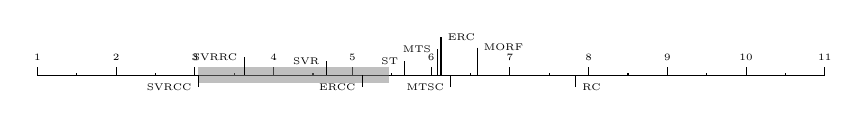
\begin{tikzpicture}
 %axis
 \draw (1,0) -- (11,0);
 \foreach \x in {1,2,3,4,5,6,7,8,9,10,11} {
  \draw (\x, 0) -- ++(0,.1) node [above,scale=0.7] {\tiny \x};
  \ifthenelse{\x < 11}{\draw (\x+.5, 0) -- ++(0,.03);}{}
 }
 % coordinates
 \coordinate (c0) at (3.0417,0);
 \coordinate (c1) at (3.6250,0);
 \coordinate (c2) at (4.6667,0);
 \coordinate (c3) at (5.1250,0);
 \coordinate (c4) at (6.1250,0);
 \coordinate (c5) at (7.8333,0);
 \coordinate (c6) at (6.2500,0);
 \coordinate (c7) at (6.0833,0);
 \coordinate (c8) at (5.6667,0);
 \coordinate (c9) at (6.5833,0);

 % labels
 \node (l0) at (c0) [below left=.025cm and 0cm, align=right,scale=0.7] {\tiny SVRCC};
 \node (l1) at (c1) [above left=.1cm and 0cm, align=right,scale=0.7] {\tiny SVRRC};
 \node (l2) at (c2) [above left=.05cm and 0cm, align=right,scale=0.7] {\tiny SVR};
 \node (l3) at (c3) [below left=.025cm and 0cm, align=left,scale=0.7] {\tiny ERCC};
 \node (l4) at (c4) [above right=.35cm and 0cm, align=right,scale=0.7] {\tiny ERC};
 \node (l5) at (c5) [below right=.025cm and 0cm, align=left,scale=0.7] {\tiny RC};
 \node (l6) at (c6) [below left=.025cm and 0cm, align=right,scale=0.7] {\tiny MTSC};
 \node (l7) at (c7) [above left=.2cm and 0cm, align=left,scale=0.7] {\tiny MTS};
 \node (l8) at (c8) [above left=.05cm and 0cm, align=right,scale=0.7] {\tiny ST};
 \node (l9) at (c9) [above right=.22cm and 0cm, align=right,scale=0.7] {\tiny MORF};

 % CD = 1.4845
 \fill[fill=gray,fill opacity=0.5] (3.0417,-0.1) rectangle (5.4653,0.1);
 
 % connectors
 \foreach \x in {0,...,9} {
  \draw (l\x) -| (c\x);
 };
\end{tikzpicture}}\vspace{-1em}
\captionof{figure}{Bonferroni-Dunn test for MSE}\label{fig:BonfDunnMSE}\vspace{-1.5em}
\captionof{table}{Wilcoxon, Nemenyi, and Holm tests for MSE}\label{tab:statmse}
\scriptsize
\resizebox{0.95\textwidth}{!}{\begin{tabular}{lccccc}
\noalign{\smallskip}\hline\noalign{\smallskip}
SVRCC vs. & Wilcoxon $R^{+}$ & Wilcoxon $R^{-}$ & Wilcoxon $p$-value & Nemenyi $p$-value & Holm $p$-value \\ 
\noalign{\smallskip}\hline\noalign{\smallskip}
MORF & 268.0 & 32.0 & $3.2E^{-4}$ & $5.1E^{-5}$ & $6.3E^{-3}$ \\
ST & 241.0 & 59.0 & $7.9E^{-3}$ & $2.7E^{-3}$ & $1.3E^{-2}$ \\
MTS & 224.0 & 76.0 & $3.4E^{-2}$ & $5.0E^{-4}$ & $1.0E^{-2}$ \\
MTSC & 226.0 & 74.0 & $2.9E^{-2}$ & $2.4E^{-4}$ & $7.1E^{-3}$ \\ 
RC & 263.0 & 37.0 & $6.5E^{-4}$ & 0.0000 & $5.6E^{-3}$ \\  
ERC & 234.0 & 66.0 & $1.5E^{-2}$ & $4.2E^{-4}$ & $8.3E^{-3}$ \\
ERCC & 224.0 & 76.0 & $3.4E^{-2}$ & $1.7E^{-2}$ & $1.7E^{-2}$ \\
SVR & 262.0 & 38.0 & $7.4E^{-4}$ & $6.3E^{-2}$ & $2.5E^{-2}$ \\ 
SVRRC & 245.0 & 55.0 & $5.3E^{-3}$ & $5.1E^{-1}$ & $5.0E^{-2}$\\ 
\noalign{\smallskip}\hline\noalign{\smallskip}
\end{tabular}}
\end{table}
\subsection{Mean Square Error}\label{subsec:mse}
Table~{\ref{tab:mseResults}} shows that our proposed methods perform the best on $15$ out of the $24$ datasets. In this case, SVRCC also performs the best on $11$ versus the $9$ that the competing methods performed better at. The Iman-Davenport statistic, distributed according to the F-distribution with $9$ and $207$ degrees of freedom is $6.57$, with a $p$-value of $3.1E^{-8}$, implying statistically significant differences among the MSE results.

Figure~{\ref{fig:BonfDunnMSE}} shows the mean rank values of each algorithm along with the critical difference value, $2.4236$, for $\alpha = 0.05$. According to the critical difference bar, there are $6$ out of $10$ algorithms beyond that perform significantly worse than our control algorithm, SVRCC. According to the Wilcoxon test, shown in Table~{\ref{tab:statmse}}, SVRCC is shown to have significantly better performance over all algorithms with $p$-value $< 0.05$. The Nemenyi and Holm tests show that SVRCC performs significantly better than $6$ out of the $9$ algorithms with $p$-values $\leq 5.6E^{-3}$ and $\leq 1.7E^{-2}$ respectively, and has an exact confidence of $0.95$ against all others.

\subsection{Average Root Mean Square Error}\label{subsec:armse}
Table~{\ref{tab:armseresults}} shows that our proposed methods perform the best on $18$ out of the $24$ datasets. In this case, SVRCC performs the best on $15$ versus the $6$ that the methods compared performed better at. The Iman-Davenport statistic is $7.6$, with a $p$-value of $1.3E^{-9}$, implying statistically significant differences in the aRMSE results.

Figure~{\ref{fig:BonfDunnaRMSE}} shows the mean rank values of each algorithm along with the critical difference value, $2.4236$, for $\alpha = 0.05$. According to the critical difference bar, there are $7$ out of $10$ algorithms that perform significantly worse than our control algorithm, SVRCC.

According to the Wilcoxon test, shown in Table~{\ref{tab:statarmse}}, SVRCC is shown to have significantly better performance over all algorithms with $p$-value $< 0.01$. The Nemenyi test shows that SVRCC performs significantly better than $7$ out of the $9$ algorithms with $p$-value $\leq 5.6E^{-3}$, while the stricter Holm test shows that it performs significantly better than $8$ out of the $9$ algorithms with $p$-value $\leq 0.05$.
\begin{table}[t!]
\centering \small
\caption{Average Root Mean Square Error (aRMSE) for MT regressors}\label{tab:armseresults}
\resizebox{0.95\textwidth}{!}{\begin{tabular}{l@{\extracolsep{\fill}}ccccccccccc}
\noalign{\smallskip}\hline\noalign{\smallskip}
Datasets &MORF &ST &MTS &MTSC &RC &ERC &ERCC &SVR &SVRRC &SVRCC \\
\noalign{\smallskip}\hline\noalign{\smallskip}
Slump &0.6711 &0.6652 &0.6456 &0.6699 &0.6787 &0.6793 &0.6649 &0.5561 &0.5345 &\textbf{0.5337} &  \\
Polymer &0.5277 &0.5409 &0.5042 &0.5336 &0.5536 &0.5803 &0.5319 &0.4403 &0.4062 &\textbf{0.4060} &  \\
Andro &0.4649 &0.5420 &0.4414 &0.4871 &0.5390 &0.5317 &0.5039 &0.4326 &0.4061 &\textbf{0.3989} &  \\
EDM &0.6372 &0.6715 &0.6705 &0.6729 &0.6722 &0.6704 &0.6721 &0.6449 &0.6411 &\textbf{0.6366} &  \\
Solar Flare 1 &0.9777 &0.9274 &0.9271 &0.9089 &0.8921 &0.9016 &0.9121 &0.8856 &0.8844 &\textbf{0.8801} &  \\
Jura &0.5800 &0.5686 &0.5720 &0.5706 &0.5726 &0.5712 &0.5693 &0.5794 &0.5687 &\textbf{0.5622} &  \\
Enb &0.1212 &0.1166 &0.1237 &0.1214 &0.1272 &0.1253 &0.1140 &0.0981 &0.0914 &\textbf{0.0903} &  \\
Solar Flare 2 &0.8725 &0.8420 &\textbf{0.8127} &0.8305 &0.8313 &0.8300 &0.8304 &0.8418 &0.8349 &0.8345 &  \\
Wisconsin Cancer &0.9290 &0.9163 &0.9158 &0.9187 &\textbf{0.9153} &0.9160 &0.9173 &0.9422 &0.9362 &0.9306 &  \\
California Housing &0.6541 &0.6366 &0.6889 &0.6530 &0.7053 &0.6632 &0.6079 &0.6038 &0.5859 &\textbf{0.5755} &  \\
Stock &0.1643 &0.1830 &0.1774 &0.1790 &0.1790 &0.1777 &0.1739 &0.1357 &0.1329 &\textbf{0.1308} &  \\
SCPF &0.7113 &0.7235 &0.7342 &0.7255 &0.7285 &0.7143 &0.7227 &0.7155 &0.7081 &\textbf{0.7048} &  \\
Puma8NH &0.7855 &0.8139 &0.8114 &0.8307 &0.8196 &0.8202 &0.8203 &\textbf{0.7650} &0.7740 &0.7671 &  \\
Friedman &0.9382 &0.9203 &0.9219 &0.9199 &0.9219 &0.9197 &0.9193 &0.9203 &0.9195 &\textbf{0.9183} &  \\
Puma32H &0.9395 &\textbf{0.8700} &0.8713 &0.8778 &0.8739 &0.8716 &0.8727 &0.9353 &0.9356 &0.9331 &  \\
Water Quality &\textbf{0.8921} &0.9015 &0.9041 &0.9025 &0.9051 &0.9030 &0.8990 &0.9284 &0.9293 &0.9271 &  \\
M5SPEC &0.5707 &0.5324 &0.5761 &0.5515 &0.5347 &0.5339 &0.5376 &0.2745 &0.2744 &\textbf{0.2740} &  \\
MP5SPEC &0.5315 &0.4914 &0.5426 &0.4947 &0.4930 &0.4928 &0.4928 &0.2337 &\textbf{0.2176} &0.2177 &  \\
MP6SPEC &0.5344 &0.4939 &0.5416 &0.4943 &0.4982 &0.4967 &0.4927 &0.2627 &\textbf{0.2460} &0.2497 &  \\
ATP7d &0.5216 &0.4956 &\textbf{0.4752} &0.4765 &0.5194 &0.5024 &0.4824 &0.5141 &0.5066 &0.5018 &  \\
OES97 &0.4652 &0.4634 &0.4635 &0.4622 &0.4643 &0.4644 &0.4627 &0.3794 &0.3768 &\textbf{0.3749} &  \\
Osales &0.7190 &0.6912 &\textbf{0.6496} &0.6615 &0.7591 &0.6772 &0.6515 &0.7212 &0.7343 &0.7121 &  \\
ATP1d &0.4053 &0.3608 &0.3587 &0.3591 &0.3653 &0.3562 &0.3596 &0.3693 &0.3638 &\textbf{0.3507} &  \\
OES10 &0.3954 &0.3896 &0.3897 &0.3892 &0.3901 &0.3903 &0.3889 &0.3085 &0.3039 &\textbf{0.3038} &  \\
\noalign{\smallskip}\hline\noalign{\smallskip}
Average &0.6254 &0.6149 &0.6133 &0.6121 &0.6225 &0.6162 &0.6083 &0.5620 &0.5547 &\textbf{0.5506} &  \\
Ranks &7.3333 &5.7708 &5.8125 &6.0625 &7.6250 &6.0208 &4.8542 &5.0625 &3.9167 &\textbf{2.5417} &  \\
\noalign{\smallskip}\hline
\end{tabular}}
\centering \small
\resizebox{0.95\textwidth}{!}{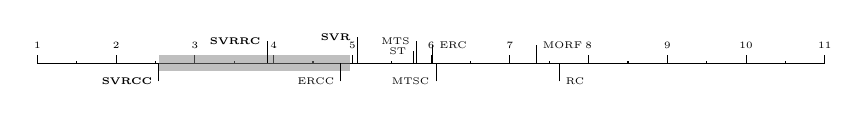
\begin{tikzpicture}
 %axis
 \draw (1,0) -- (11,0);
 \foreach \x in {1,2,3,4,5,6,7,8,9,10,11} {
  \draw (\x, 0) -- ++(0,.1) node [above,scale=0.7] {\tiny \x};
  \ifthenelse{\x < 11}{\draw (\x+.5, 0) -- ++(0,.03);}{}
 }
 % coordinates
 \coordinate (c0) at (2.5417,0);
 \coordinate (c1) at (3.9167,0);
 \coordinate (c2) at (5.0625,0);
 \coordinate (c3) at (4.8542,0);
 \coordinate (c4) at (6.0208,0);
 \coordinate (c5) at (7.6250,0);
 \coordinate (c6) at (6.0625,0);
 \coordinate (c7) at (5.8125,0);
 \coordinate (c8) at (5.7708,0);
 \coordinate (c9) at (7.3333,0);

 % labels
 \node (l0) at (c0) [below left=.1cm and 0cm, align=right,scale=0.7] {\tiny \textbf{SVRCC}};
 \node (l1) at (c1) [above left=.15cm and 0cm, align=right,scale=0.7] {\tiny \textbf{SVRRC}};
 \node (l2) at (c2) [above left=.2cm and 0cm, align=right,scale=0.7] {\tiny \textbf{SVR}};
 \node (l3) at (c3) [below left=.1cm and 0cm, align=left,scale=0.7] {\tiny ERCC};
 \node (l4) at (c4) [above right=.1cm and 0cm, align=right,scale=0.7] {\tiny ERC};
 \node (l5) at (c5) [below right=.1cm and 0cm, align=left,scale=0.7] {\tiny RC};
 \node (l6) at (c6) [below left=.1cm and 0cm, align=right,scale=0.7] {\tiny MTSC};
 \node (l7) at (c7) [above left=.15cm and 0cm, align=left,scale=0.7] {\tiny MTS};
 \node (l8) at (c8) [above left=.025cm and 0cm, align=right,scale=0.7] {\tiny ST};
 \node (l9) at (c9) [above right=.1cm and 0cm, align=right,scale=0.7] {\tiny MORF};

 % CD = 1.4845
 \fill[fill=gray,fill opacity=0.5] (2.5417,-0.1) rectangle (4.9653,0.1);
 
 % connectors
 \foreach \x in {0,...,9} {
  \draw (l\x) -| (c\x);
 };
\end{tikzpicture}}\vspace{-1em}
\captionof{figure}{Bonferroni-Dunn test for aRMSE}\label{fig:BonfDunnaRMSE}\vspace{-1.5em}
\captionof{table}{Wilcoxon, Nemenyi, and Holm tests for aRMSE}\label{tab:statarmse}
\scriptsize
\resizebox{0.95\textwidth}{!}{\begin{tabular}{lccccc}
\noalign{\smallskip}\hline\noalign{\smallskip}
SVRCC vs. & Wilcoxon $R^{+}$ & Wilcoxon $R^{-}$ & Wilcoxon $p$-value & Nemenyi $p$-value & Holm $p$-value \\ 
\noalign{\smallskip}\hline\noalign{\smallskip}
MORF & 286.0 & 14.0 & $1.3E^{-5}$ & 0.0000 & $6.3E^{-3}$ \\
ST & 259.0 & 41.0 & $1.1E^{-3}$ & $2.2E^{-4}$ & $1.3E^{-2}$ \\
MTS & 247.0 & 53.0 & $4.3E^{-3}$ & $1.8E^{-5}$ & $1.0E^{-2}$ \\ 
MTSC & 251.0 & 49.0 & $2.8E^{-3}$ & $5.6E^{-5}$ & $7.1E^{-3}$ \\
RC & 270.0 & 30.0 & $2.4E^{-4}$ & 0.0000 & $5.6E^{-3}$ \\ 
ERC & 255.0 & 45.0 & $1.8E^{-3}$ & $6.9E^{-5}$ & $8.3E^{-3}$ \\
ERCC & 246.0 & 54.0 & $4.8E^{-3}$ & $8.2E^{-3}$ & $2.5E^{-2}$ \\
SVR & 296.0 & 4.00 & $8.3E^{-7}$ & $3.9E^{-3}$ & $1.7E^{-2}$ \\
SVRRC & 284.0 & 16.0 & $2.0E^{-5}$ & $1.2E^{-1}$ & $5.0E^{-2}$ \\
\noalign{\smallskip}\hline\noalign{\smallskip}
\end{tabular}}
\end{table}

\subsection{Average Relative Root Mean Square Error}\label{subsec:arrmse}
\begin{table}[b!]
\centering \small
\caption{Average Relative Root Mean Square Error (aRRMSE) for MT regressors}\label{tab:arrmseresults}
\resizebox{0.95\textwidth}{!}{\begin{tabular}{l@{\extracolsep{\fill}}ccccccccccc}
\noalign{\smallskip}\hline\noalign{\smallskip}
Datasets &MORF &ST &MTS &MTSC &RC &ERC &ERCC &SVR &SVRRC &SVRCC \\
\noalign{\smallskip}\hline\noalign{\smallskip}
Slump &0.6939 &0.6886 &0.6690 &0.6938 &0.7019 &0.7022 &0.6886 &0.5765 &\textbf{0.5545} &0.5560 &  \\
Polymer &0.6159 &0.5971 &0.5778 &0.6493 &0.6270 &0.6544 &0.6131 &0.5573 &0.5253 &\textbf{0.5116} &  \\
Andro &0.5097 &0.5979 &0.5155 &0.5633 &0.5924 &0.5885 &0.5666 &0.4856 &0.4651 &\textbf{0.4455} &  \\
EDM &0.7337 &0.7442 &0.7413 &0.7446 &0.7449 &0.7452 &0.7443 &0.7058 &0.7070 &\textbf{0.6978} &  \\
Solar Flare 1 &1.3046 &1.1357 &1.1168 &1.0758 &0.9951 &1.0457 &1.0887 &0.9917 &0.9455 &\textbf{0.9320} &  \\
Jura &0.5969 &0.5874 &0.5906 &0.5892 &0.5910 &0.5896 &0.5880 &0.5952 &\textbf{0.5764} &0.5885 &  \\
Enb &0.1210 &0.1165 &0.1231 &0.1211 &0.1268 &0.1250 &0.1139 &0.0977 &0.0910 &\textbf{0.0899} &  \\
Solar Flare 2 &1.4167 &1.1503 &\textbf{0.9483} &1.0840 &1.0092 &1.0522 &1.0928 &1.0385 &1.0253 &1.0298 &  \\
Wisconsin Cancer &0.9413 &0.9314 &0.9308 &0.9336 &\textbf{0.9305} &0.9313 &0.9323 &0.9555 &0.9483 &0.9427 &  \\
California Housing &0.6611 &0.6447 &0.6974 &0.6630 &0.7131 &0.6690 &0.6146 &0.6130 &0.5945 &\textbf{0.5852} &  \\
Stock &0.1653 &0.1844 &0.1787 &0.1803 &0.1802 &0.1789 &0.1752 &0.1364 &\textbf{0.1337} &0.1388 &  \\
SCPF &0.8273 &0.8348 &0.8436 &0.8308 &0.8263 &0.8105 &0.8290 &0.8164 &0.8037 &\textbf{0.8013} &  \\
Puma8NH &0.7858 &0.8142 &0.8118 &0.8311 &0.8199 &0.8205 &0.8207 &\textbf{0.7655} &0.7744 &0.7676 &  \\
Friedman &0.9394 &0.9214 &0.9231 &0.9210 &0.9231 &0.9209 &0.9204 &0.9218 &0.9208 &\textbf{0.9196} &  \\
Puma32H &0.9406 &\textbf{0.8713} &0.8727 &0.8791 &0.8752 &0.8729 &0.8740 &0.9364 &0.9367 &0.9319 &  \\
Water Quality &\textbf{0.8994} &0.9085 &0.9109 &0.9093 &0.9121 &0.9097 &0.9057 &0.9343 &0.9310 &0.9045 &  \\
M5SPEC &0.5910 &0.5523 &0.5974 &0.5671 &0.5552 &0.5542 &0.5558 &0.2951 &0.2935 &\textbf{0.2925} &  \\
MP5SPEC &0.5522 &0.5120 &0.5683 &0.5133 &0.5145 &0.5143 &0.5119 &0.2484 &\textbf{0.2323} &0.2358 &  \\
MP6SPEC &0.5553 &0.5152 &0.5686 &0.5119 &0.5198 &0.5187 &0.5109 &0.2850 &0.2669 &\textbf{0.2623} &  \\
ATP7d &0.5563 &0.5308 &\textbf{0.5141} &0.5142 &0.5558 &0.5397 &0.5182 &0.5455 &0.5371 &0.5342 &  \\
OES97 &0.5490 &0.5230 &0.5229 &0.5217 &0.5239 &0.5237 &0.5222 &0.4641 &\textbf{0.4618} &0.4635 &  \\
Osales &0.7596 &0.7471 &\textbf{0.7086} &0.7268 &0.8318 &0.7258 &0.7101 &0.7924 &0.7924 &0.7811 &  \\
ATP1d &0.4173 &0.3732 &0.3733 &0.3712 &0.3790 &\textbf{0.3696} &0.3721 &0.3773 &0.3707 &0.3775 &  \\
OES10 &0.4518 &0.4174 &0.4176 &0.4171 &0.4178 &0.4180 &0.4166 &0.3570 &0.3555 &\textbf{0.3538} &  \\
\noalign{\smallskip}\hline\noalign{\smallskip}
Average &0.6910 &0.6625 &0.6551 &0.6589 &0.6611 &0.6575 &0.6536 &0.6039 &0.5935 &\textbf{0.5893} &  \\
Ranks &7.5000 &5.7708 &5.9375 &6.1667 &7.4375 &6.3750 &4.9792 &4.7708 &3.2708 &\textbf{2.7917} &  \\
\noalign{\smallskip}\hline
\end{tabular}}
\centering \small
\resizebox{0.95\textwidth}{!}{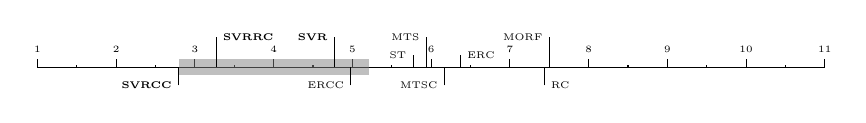
\begin{tikzpicture}
 %axis
 \draw (1,0) -- (11,0);
 \foreach \x in {1,2,3,4,5,6,7,8,9,10,11} {
  \draw (\x, 0) -- ++(0,.1) node [above,scale=0.7] {\tiny \x};
  \ifthenelse{\x < 11}{\draw (\x+.5, 0) -- ++(0,.03);}{}
 }
 % coordinates
 \coordinate (c0) at (2.7917,0);
 \coordinate (c1) at (3.2708,0);
 \coordinate (c2) at (4.7708,0);
 \coordinate (c3) at (4.9792,0);
 \coordinate (c4) at (6.3750,0);
 \coordinate (c5) at (7.4375,0);
 \coordinate (c6) at (6.1667,0);
 \coordinate (c7) at (5.9375,0);
 \coordinate (c8) at (5.7708,0);
 \coordinate (c9) at (7.5000,0);

 % labels
 \node (l0) at (c0) [below left=.1cm and 0cm, align=right,scale=0.7] {\tiny \textbf{SVRCC}};
 \node (l1) at (c1) [above right=.25cm and 0cm, align=right,scale=0.7] {\tiny \textbf{SVRRC}};
 \node (l2) at (c2) [above left=.25cm and 0cm, align=right,scale=0.7] {\tiny \textbf{SVR}};
 \node (l3) at (c3) [below left=.1cm and 0cm, align=left,scale=0.7] {\tiny ERCC};
 \node (l4) at (c4) [above right=.025cm and 0cm, align=right,scale=0.7] {\tiny ERC};
 \node (l5) at (c5) [below right=.1cm and 0cm, align=left,scale=0.7] {\tiny RC};
 \node (l6) at (c6) [below left=.1cm and 0cm, align=right,scale=0.7] {\tiny MTSC};
 \node (l7) at (c7) [above left=.25cm and 0cm, align=left,scale=0.7] {\tiny MTS};
 \node (l8) at (c8) [above left=.025cm and 0cm, align=right,scale=0.7] {\tiny ST};
 \node (l9) at (c9) [above left=.25cm and 0cm, align=right,scale=0.7] {\tiny MORF};

 % CD = 1.4845
 \fill[fill=gray,fill opacity=0.5] (2.7917,-0.1) rectangle (5.2153,0.1);
 
 % connectors
 \foreach \x in {0,...,9} {
  \draw (l\x) -| (c\x);
 };
\end{tikzpicture}}\vspace{-1em}
\captionof{figure}{Bonferroni-Dunn test for aRRMSE}\label{fig:BonfDunnaRRMSE}\vspace{-1.5em}
\captionof{table}{Wilcoxon, Nemenyi, and Holm tests for aRRMSE}\label{tab:statarrmse}
\scriptsize
\resizebox{0.95\textwidth}{!}{\begin{tabular}{lccccc}
\noalign{\smallskip}\hline\noalign{\smallskip}
SVRCC vs. & Wilcoxon $R^{+}$ & Wilcoxon $R^{-}$ & Wilcoxon $p$-value & Nemenyi $p$-value & Holm $p$-value \\ 
\noalign{\smallskip}\hline\noalign{\smallskip}
MORF & 290.0 & 10.0 & $5.1E^{-6}$ & $0.0000$ & $5.6E^{-3}$ \\  
ST & 261.0 & 39.0 & $8.5E^{-4}$ & $6.5E^{-4}$ & $1.3E^{-2}$\\
MTS & 239.0 & 61.0 & $9.6E^{-3}$ & $3.2E^{-3}$ & $1.0E^{-2}$\\ 
MTSC & 261.0 & 39.0 & $8.5E^{-4}$ & $1.1E^{-3}$ & $8.3E^{-3}$\\  
RC & 275.0 & 25.0 & $1.1E^{-4}$ & 0.0000 & $6.3E^{-3}$ \\
ERC & 261.0 & 39.0 & $8.5E^{-4}$ & $4.1E^{-5}$ & $7.1E^{-3}$\\ 
ERCC & 254.0 & 46.0 & $2.0E^{-3}$ & $1.2E^{-2}$ & $1.7E^{-2}$\\
SVR & 291.0 & 9.00 & $3.9E^{-6}$ & $2.4E^{-2}$ & $2.5E^{-2}$\\
SVRRC & 222.5 & 77.5 & $3.8E^{-2}$ & $5.8E^{-1}$ & $5.0E^{-2}$ \\ 
\noalign{\smallskip}\hline\noalign{\smallskip}
\end{tabular}}
\end{table}
Table~{\ref{tab:arrmseresults}} shows that our proposed methods perform the best on $16$ out of the $24$ datasets. In this case, SVRCC performs the best on $11$ versus the $6$ that the competing methods performed better at. The Iman-Davenport statistic is $8.54$, with a $p$-value of $7.6E^{-11}$.

Figure~{\ref{fig:BonfDunnaRRMSE}} shows the mean rank values of each algorithm along with the critical difference value, $2.4236$, for $\alpha = 0.05$. According to the critical difference bar, there are $6$ out of $10$ algorithms beyond that perform significantly worse than our control algorithm, SVRCC.

According to the Wilcoxon test, shown in Table~{\ref{tab:statarrmse}}, SVRCC is shown to have significantly better performance over all algorithms with $p$-value $< 0.05$, and $8$ out of the $9$ algorithms for $p$-value $< 0.01$. The Nemenyi test shows that SVRCC performs significantly better than $6$ out of the $9$ algorithms with $p$-value $\leq 5.6E^{-3}$, and the Holm test shows its performance is significantly better than $8$ out of the $9$ algorithms with $p$-value $\leq 0.05$.

\subsection{Run Time}\label{subsec:time}
\begin{table}[t!]
\centering \small
\caption{Run Time (seconds) for MT regressors}\label{tab:timeresults}
\resizebox{0.95\textwidth}{!}{\begin{tabular}{l@{\extracolsep{\fill}}rrrrrrrrrrr}
\noalign{\smallskip}\hline\noalign{\smallskip}
Datasets &MORF &ST &MTS &MTSC &RC &ERC &ERCC &SVR &SVRRC &SVRCC \\
\noalign{\smallskip}\hline\noalign{\smallskip}
Slump &38.1 &2.6 &9.9 &15.9 &1.8 &11.1 &50.5 &\textbf{0.6} &1.9 &0.7 &  \\
Polymer &7.6 &2.7 &9.1 &15.5 &1.9 &14.9 &80.5 &\textbf{0.5} &2.6 &\textbf{0.5} &  \\
Andro &25.7 &4.4 &15.0 &34.2 &3.4 &33.2 &197.9 &\textbf{1.1} &6.2 &\textbf{1.1} &  \\
EDM &24.8 &2.8 &9.4 &18.1 &2.1 &5.8 &19.0 &\textbf{0.9} &1.0 &\textbf{0.9} &  \\
Solar Flare 1 &34.1 &3.5 &13.6 &26.7 &2.7 &17.7 &86.9 &\textbf{2.3} &9.3 &2.6 &  \\
Jura &64.3 &7.9 &31.8 &74.3 &6.4 &43.5 &254.2 &\textbf{4.7} &18.7 &5.3 &  \\
Enb &71.4 &6.6 &26.1 &63.6 &\textbf{5.4} &15.6 &69.6 &11.3 &17.7 &15.9 &  \\
Solar Flare 2 &55.4 &7.4 &30.7 &68.0 &\textbf{6.3} &42.9 &241.5 &9.4 &53.5 &15.6 &  \\
Wisconsin Cancer &51.4 &6.1 &21.9 &53.7 &4.9 &14.8 &61.6 &\textbf{2.0} &2.4 &\textbf{2.0} &  \\
California Housing &93.0 &9.7 &34.8 &75.9 &\textbf{8.2} &21.3 &102.0 &15.8 &25.2 &23.6 &  \\
Stock &93.7 &11.7 &46.8 &96.7 &\textbf{11.0} &75.4 &427.3 &18.5 &90.5 &26.3 &  \\
SCPF &66.3 &19.3 &65.9 &176.3 &\textbf{15.0} &104.2 &734.2 &32.8 &162.8 &48.8 &  \\
Puma8NH &130.4 &29.7 &106.7 &288.6 &\textbf{27.9} &201.6 &1227.7 &94.1 &516.6 &177.1 &  \\
Friedman &79.5 &27.0 &81.2 &258.3 &25.0 &273.7 &2871.6 &\textbf{12.3} &322.3 &18.8 &  \\
Puma32H &93.9 &68.1 &181.0 &635.0 &87.7 &667.9 &6087.0 &\textbf{32.2} &1018.7 &53.1 &  \\
Water Quality &108.4 &\textbf{93.1} &262.1 &912.3 &127.2 &925.4 &10993.3 &110.2 &2567.9 &189.5 &  \\
M5SPEC &89.8 &68.9 &166.3 &604.6 &73.7 &262.3 &3132.1 &\textbf{39.2} &546.7 &45.1 &  \\
MP5SPEC &84.5 &94.6 &221.2 &888.3 &91.5 &557.0 &6864.1 &\textbf{49.3} &1132.1 &58.4 &  \\
MP6SPEC &90.3 &93.4 &212.6 &871.0 &89.1 &557.6 &6761.3 &\textbf{47.2} &1227.1 &58.5 &  \\
ATP7d &\textbf{70.5} &262.6 &452.1 &2319.8 &242.1 &1779.2 &24373.8 &80.0 &1897.4 &136.5 &  \\
OES97 &\textbf{83.4} &485.3 &1146.6 &4928.9 &499.8 &5315.0 &58072.1 &148.2 &3759.1 &342.6 &  \\
Osales &\textbf{92.0} &1094.8 &2340.7 &8322.2 &986.5 &11361.2 &122265.3 &437.0 &4830.1 &843.6 &  \\
ATP1d &\textbf{70.7} &272.9 &476.5 &2568.9 &261.9 &2138.9 &26768.9 &95.0 &2127.8 &174.4 &  \\
OES10 &\textbf{90.0} &738.9 &1633.6 &6682.9 &688.5 &7150.8 &83533.1 &229.1 &5419.4 &577.1 &  \\
\noalign{\smallskip}\hline\noalign{\smallskip}
Average &71.2 &142.2 &316.5 &1250.0 &136.2 &1316.3 &14803.2 &\textbf{61.4} &1073.2 &117.4 &  \\
Ranks &5.5 &3.71 &6.0 &8.29 &3.0 &7.08 &9.92 &\textbf{1.88} &6.71 &2.92 &  \\
\noalign{\smallskip}\hline
\end{tabular}}
\centering \small
\resizebox{0.95\textwidth}{!}{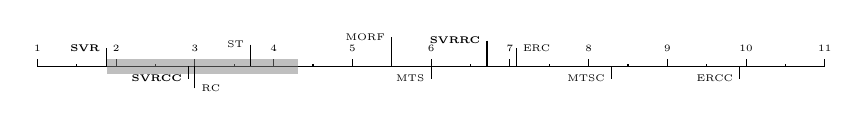
\begin{tikzpicture}
 %axis
 \draw (1,0) -- (11,0);
 \foreach \x in {1,2,3,4,5,6,7,8,9,10,11} {
  \draw (\x, 0) -- ++(0,.1) node [above,scale=0.7] {\tiny \x};
  \ifthenelse{\x < 11}{\draw (\x+.5, 0) -- ++(0,.03);}{}
 }
 % coordinates
 \coordinate (c0) at (2.92,0);
 \coordinate (c1) at (6.71,0);
 \coordinate (c2) at (1.88,0);
 \coordinate (c3) at (9.92,0);
 \coordinate (c4) at (7.08,0);
 \coordinate (c5) at (3,0);
 \coordinate (c6) at (8.29,0);
 \coordinate (c7) at (6,0);
 \coordinate (c8) at (3.71,0);
 \coordinate (c9) at (5.5,0);

 % labels
 \node (l0) at (c0) [below left=.025cm and 0cm, align=right,scale=0.7] {\tiny \textbf{SVRCC}};
 \node (l1) at (c1) [above left=.2cm and 0cm, align=right,scale=0.7] {\tiny \textbf{SVRRC}};
 \node (l2) at (c2) [above left=.1cm and 0cm, align=right,scale=0.7] {\tiny \textbf{SVR}};
 \node (l3) at (c3) [below left=.025cm and 0cm, align=left,scale=0.7] {\tiny ERCC};
 \node (l4) at (c4) [above right=.1cm and 0cm, align=right,scale=0.7] {\tiny ERC};
 \node (l5) at (c5) [below right=.15cm and 0cm, align=left,scale=0.7] {\tiny RC};
 \node (l6) at (c6) [below left=.025cm and 0cm, align=right,scale=0.7] {\tiny MTSC};
 \node (l7) at (c7) [below left=.025cm and 0cm, align=left,scale=0.7] {\tiny MTS};
 \node (l8) at (c8) [above left=.15cm and 0cm, align=right,scale=0.7] {\tiny ST};
 \node (l9) at (c9) [above left=.24cm and 0cm, align=right,scale=0.7] {\tiny MORF};

 % CD = 1.4845
 \fill[fill=gray,fill opacity=0.5] (1.88,-0.1) rectangle (4.3036,0.1);
 
 % connectors
 \foreach \x in {0,...,9} {
  \draw (l\x) -| (c\x);
 };
\end{tikzpicture}}\vspace{-1em}
\captionof{figure}{Bonferroni-Dunn test for Run Time}\label{fig:BonfDunnTime}\vspace{-1.5em}
\captionof{table}{Wilcoxon, Nemenyi, and Holm tests for Run Time}\label{tab:stattime}
\scriptsize
\resizebox{0.95\textwidth}{!}{\begin{tabular}{lccccc}
\noalign{\smallskip}\hline\noalign{\smallskip}
SVRCC vs. & Wilcoxon $R^{+}$ & Wilcoxon $R^{-}$ & Wilcoxon $p$-value & Nemenyi $p$-value & Holm $p$-value \\ 
\noalign{\smallskip}\hline\noalign{\smallskip}
SVRCC & 295.0 & 5.00 & $1.2E^{-6}$ &  $2.3E^{-1}$ & $5.0E^{-2}$\\ 
MORF & 225.0 & 75.0 & $3.2E^{-2}$ &  $3.4E^{-5}$ & $1.3E^{-2}$\\  
ST & 221.5 & 78.5 & $4.1E^{-2}$ &  $3.6E^{-2}$ & $1.7E^{-2}$\\   
MTS & 300.0 & 0.00 & $1.2E^{-7}$ &  $2.0E^{-6}$ & $1.0E^{-2}$\\ 
MTSC & 300.0 & 0.00 & $1.2E^{-7}$ &  0.0000 & $6.3E^{-3}$\\
RC & 229.0 & 71.0 & $2.3E^{-2}$ &  $2.0E^{-1}$ & $2.5E^{-2}$ \\  
ERC & 300.0 & 0.00 & $1.2E^{-7}$ & 0.0000 & $7.1E^{-3}$\\  
ERCC & 300.0 & 0.00 & $1.2E^{-7}$ & 0.0000 & $5.6E^{-3}$\\ 
SVRRC & 300.0 & 0.00 & $1.2E^{-7}$ &  0.0000 & $8.3E^{-3}$\\ 
\noalign{\smallskip}\hline\noalign{\smallskip}
\end{tabular}}
\end{table}
Table~{\ref{tab:timeresults}} shows that our proposed methods perform faster on $16$ out of the $24$ datasets. In this case, SVR performs the best on $12$ versus the $6$ of the state-of-the-art methods. The Iman-Davenport statistic $64.41$, with a $p$-value of $0.0$ which implies a statistical confidence of $100\%$. Figure~{\ref{fig:BonfDunnTime}} shows the mean rank values of each algorithm along with the critical difference value, $2.4236$, for $\alpha = 0.05$. According to the critical difference bar, there are $6$ out of $10$ algorithms beyond that perform significantly worse than our control algorithm, SVR.
According to the Wilcoxon test, shown in Table~{\ref{tab:stattime}}, SVR is shown to have significantly better performance over all algorithms with $p$-value $< 0.01$. The Nemenyi and Holm tests show that SVRCC performs significantly better than $6$ out of the $9$ algorithms and $8$ out of the $9$ algorithms with $p$-value $\leq 5.6E^{-3}$ and $p$-value $\leq 1.6E^{-2}$, respectively.

\subsection{Discussion}\label{sec:discussion}
Results indicate that our proposed methods perform competitively against the current contemporary methods, specifically SVRCC which exploits relationships among the targets. Firstly, they show that using SVR as a base-line method for multi-target chaining causes a performance improvement in model prediction, compared to other ST base-line models, as well as most MT methods. This demonstrates the advantages of using the SVR method as a base-line for multi-target learning, thus increasing the performance of the ensemble of regressor chains, SVRRC, compared to ERCC. More importantly, the results highlight the major advantage of capturing and exploiting the targets' relationships during model training. Using an ensemble of randomly generated chains does not ensure the targets' correlations are fully captured; however, using a maximum correlation chain improves the performance in terms of quality metrics as well as run time. The run time of SVR was shown to be the fastest, due to the fact that its complexity is mostly dependent on the number of targets. However, this method does not consider any of the correlations that might exist among the target variables, but SVRCC does take them into account and does not have a significant impact on run time. The most noteworthy finding that highlights advantage of using the base-line SVR and the maximum correlation method, SVRCC, rather than random chaining as done in ERCC, are the run time results and their analysis. ERCC had the worst run time across all datasets, whereas our proposals, SVR and SVRCC, performed the fastest. This emphasizes the advantage of using a single chain rather an ensemble of random chains, especially when the single chain is ordered in the direction of the targets maximum correlation.

\section{Conclusions}\label{sec:MTRconclusions}
This contribution proposed three novel methods for solving multi-target regression problems. The first method takes a \textit{problem transformation} approach, which generates $m$ ST models, each trained independently. This base-line approach was shown to perform the best in terms of run time, but its drawback  is that it does not take the possible correlations between the target variables into account during training. The second implements SVR as an ensemble model of randomly generated chains, inspired by the classification method ERCC. This was done to investigate the effects of exploiting correlations among the target variables during model training. Due to the random nature of this method, capturing target correlations is not guaranteed. The third proposal, SVRCC, generates a single chain that is ordered in the direction of the targets' maximum correlation, ensuring the correlations among targets are taken into account within the learning process.

The experimental study compared the proposed methods' performances to $7$ popular, contemporary methods on 24 MT regression datasets. Firstly, the results show the superior performance of using the SVR method as a base-line model, rather than regression trees as used in MORF. The results for SVRRC show an increase in performance when random chaining is used to develop an ensemble model. This indicates the importance of the relationship among the target variables during training. Finally, the results show the superiority of using the SVRCC method, which was ranked the best in all quality metrics and second best in terms of run time. SVRCC performed better than the single-target SVR model and the randomly chained ensemble model SVRRC, showing that the targets' maximum correlation does positively contribute toward model training. The statistical analysis supports and shows the significance of the results obtained by our experiments. They demonstrated that statistically significant differences exist between the proposed algorithms against the methods compared. SVRCCs competitive performance, as well as speed, shows that it is a powerful learning algorithm for multi-target problems. The research outcomes of this chapter have been published in~\cite{melki2017multi}.



\end{document}